% @author Marcel Ruland (2018)

%% tell TeXshop to compile using LuaLaTeX and encode with UTF-8
%!TEX TS-program = lualatex
%!TEX encoding = UTF-8 Unicode

\documentclass[
	fontsize=11,			% font size 11pt (KOMA default)
	DIV=calc,				% KOMA calculates Satzspiegel
	BCOR=0mm,				% length that will get swallowed up by binding
	pagesize,				% ensures compatibility with PDF and DVI
	toc=bib,				% include bib in toc
	toc=listof,				% include list of tables and list of figures in toc
	abstract=true,			% display abstract heading
	twoside,				% two-sided printing
	titlepage=firstiscover,	% set title page as cover page
	footnotes=multiple		% separate footnotes set directly one after another by a comma
]{scrreprt}

\usepackage{../scrreprt/ba_style}  % loading packages, typesetting, etc.

\begin{document}
\begin{figure}
	\centering
	\input{../aux/tikzpictures/tikz_idealseq.tex}
	\caption{fig:idealseq}
	\label{fig:idealseq}
\end{figure}

\begin{figure}
	\centering
	% !TEX root = ../../scrreprt/ba_scrreprt_master.tex
% @author Marcel Ruland (2018)
\begin{tikzpicture}[
		every node/.append style={
			font=\sffamily\addfontfeature{Numbers=Lining}
		},
		node distance=2cm and 2cm
	]
%	\draw[help lines, dashed] (0,0) grid (11,4);
	
	% arrows
	\draw[vecArrow] (0,3) to node {\scriptsize\texttt{speech}} (2,3);
	\draw[vecArrow] (2.5,2) to node {\scriptsize\texttt{speech}} (4.5,2);
	\draw[vecArrow] (6.5,3) to node {\scriptsize\texttt{multimodal}} (10.5,3);
	\draw[vecArrow] (7,2) to node {\scriptsize\texttt{multimodal}} (11,2);
	
	% gaps
	\draw[stealth-stealth] (2,1) to node[above] {\tiny gap} (2.5,1);
	\draw[stealth-stealth] (6.5,1) to node[above] {\tiny gap} (7,1);
	
	% dashed lines
	\draw[dashed] (2,0.5) to (2,4);
	\draw[dashed] (2.5,0.5) to (2.5,4);
	\draw[dashed] (6.5,0.5) to (6.5,4);
	\draw[dashed] (7,0.5) to (7,4);
	
	% faces
	\node at (-1,3) {
\includegraphics[height=0.7cm]{../aux/img/child.png}};
	\node at (-1,2) {\includegraphics[height=1cm]{../aux/img/woman.png}};
	
	% annotations
	\node at (2.5,4.5) {\citet{levinson16}};
	\node at (8.5,4.5) {present thesis};
\end{tikzpicture}
	\caption{fig:levinson}
	\label{fig:levinson}
\end{figure}

\begin{figure}
	\centering
	% !TEX root = ../../scrreprt_figures/ba_scrreprt_figures.tex
% @author Marcel Ruland (2018)
\begin{tikzpicture}
	[every node/.append style={font=\sffamily\addfontfeature{Numbers=Lining}},
	node distance=1cm and 3cm,
	rounded corners,
	align=center,
	>=stealth']
	
	% nodes
	\node [draw] (sig) {\citeauthor{rohlfing18} + \\ significance};
	\node [draw, right=of sig] (reacsig) {\textsc{rt}-data + \\ significance};
	\node [draw, below=of sig] (origin) {\citeauthor{rohlfing18}};
	\node [draw, below=of reacsig] (reac) {\textsc{rt}-data};
	
	% arrows
	\draw [->] (origin) -- node[above] {\footnotesize consider reaction times} (reac);
	\draw [->] (origin) -- node[left]  {\footnotesize establish significance}  (sig);
	\draw [->] (reac)   -- node[right] {\footnotesize establish significance}  (reacsig);
	
	% discussion
%	\node [above right=of reacsig.north west] (discuss) {\footnotesize\textit{3.~extensive discussion}};
	\node at (7.5,1.61) (discuss) {\footnotesize\textit{3.~extensive discussion}};
	\draw[<->, double] (sig.north) to[bend left] node[above]{\footnotesize\textit{2.~comparison}} (reacsig.north);
	\draw[<->, double] (origin.south) to[bend right] node[below]{\footnotesize\textit{1.~comparison}} (reac.south);
	\draw[->, double] (discuss) to (reacsig.north east);
\end{tikzpicture}

















































	\caption{fig:method}
	\label{fig:method}
\end{figure}

\begin{figure}
	\centering
	% !TEX root = ../../scrreprt_figures/ba_scrreprt_figures.tex
% @author Marcel Ruland (2018)

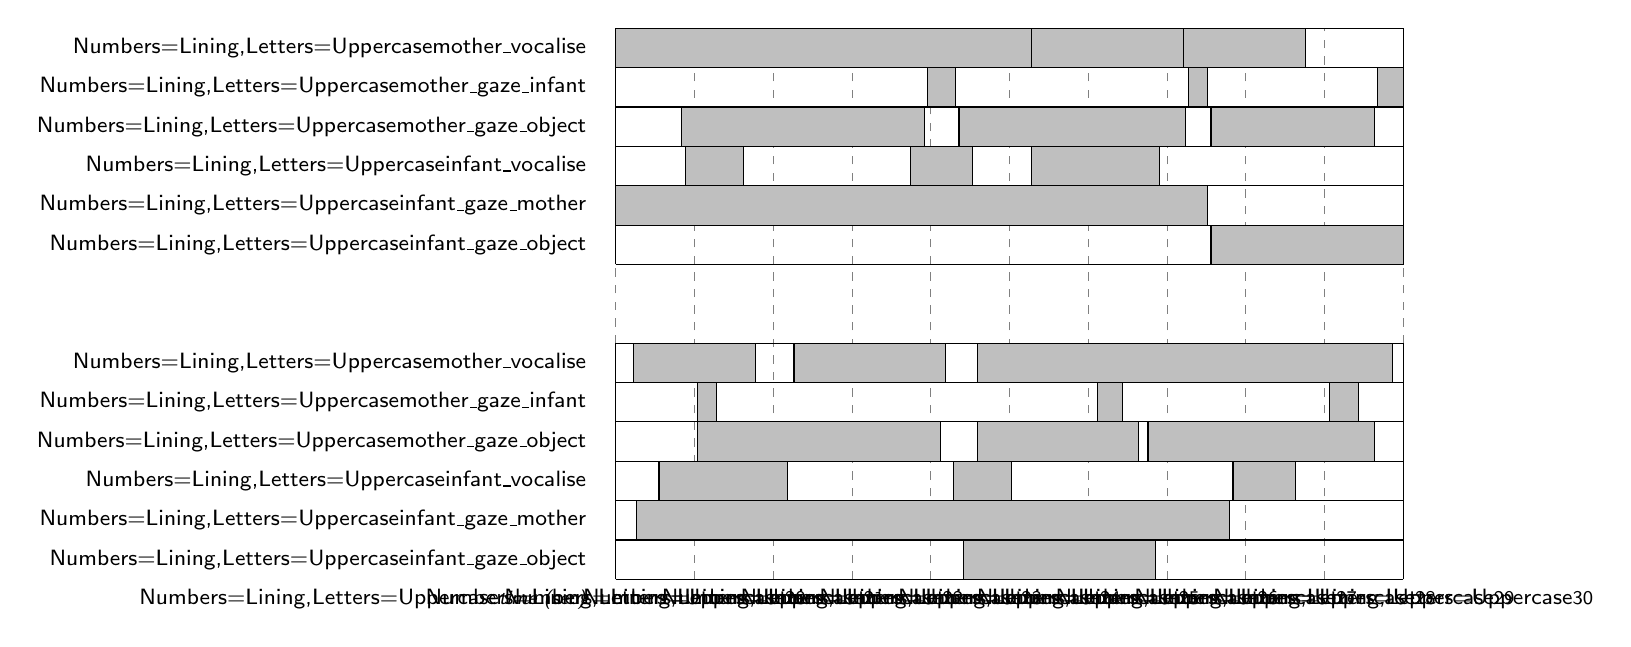
\begin{tikzpicture}[
	node distance=0 and 0,  % y, x for fuck knows what reason
	every node/.append style={font=\footnotesize\sffamily\addfontfeature{Numbers=Lining,Letters=Uppercase}}]
%	\draw [help lines, dashed] (0,0) grid (13,7);
	
	% time line
	% annotations
	\node [anchor=east] at (2.75, -0.25) {\textit{\scriptsize{time (sec)}}};
	\foreach \i in {20, 21,..., 29, 30}
		\node at ({\i-17},-0.25) {\scriptsize{\i}};
	% small vertical help lines
	\draw [help lines, dashed] (3,3) -- (3,4);
	\draw [help lines, dashed] (13,3) -- (13,4);
	% long vertical help lines
	\foreach \i in {4, 5,..., 11, 12}
		\draw [help lines, dashed] (\i,0) -- (\i,7);
	
	%% grids
	% vertical lines
	\foreach \i in {3, 13}{
		\draw (\i,4) -- (\i,7);  % top
		\draw (\i,0) -- (\i,3);  % bottom
	}
	% horizontal lines
	\foreach \i in {0, 0.5,..., 2.5, 3, 4, 4.5,..., 6.5, 7}  % top and bottom
		\draw (3,\i) -- (13,\i);
%	% annotations, not happy with them the way they are
%	\node[rotate=-90, anchor=south] at (13,5.5) {\textsc{real}};
%	\node[rotate=-90, anchor=south] at (13,1.5) {\textsc{null}};
		
	%% labels
	\foreach \i in {0.25, 4.25}{  % top and bottom
		\node[anchor=east] at (2.75,{\i+2.5}) {\code{mother\_vocalise}};
		\node[anchor=east] at (2.75,{\i+2}) {\code{mother\_gaze\_infant}};
		\node[anchor=east] at (2.75,{\i+1.5}) {\code{mother\_gaze\_object}};
		\node[anchor=east] at (2.75,{\i+1}) {\code{infant\_vocalise}};
		\node[anchor=east] at (2.75,{\i+0.5}) {\code{infant\_gaze\_mother}};
		\node[anchor=east] at (2.75,\i) {\code{infant\_gaze\_object}};
	}
	
	%% annotations
	% top
	\draw [fill=lightgray] (3,6.5) rectangle (8.279,7);
	\draw [fill=lightgray] (8.279,6.5) rectangle (10.206,7);
	\draw [fill=lightgray] (10.206,6.5) rectangle (11.76,7);

	\draw [fill=lightgray] (6.96,6) rectangle (7.32,6.5);
	\draw [fill=lightgray] (10.28,6) rectangle (10.52,6.5);
	\draw [fill=lightgray] (12.68,6) rectangle (13,6.5);
	
	\draw [fill=lightgray] (3.84,5.5) rectangle (6.92,6);
	\draw [fill=lightgray] (7.36,5.5) rectangle (10.24,6);
	\draw [fill=lightgray] (10.56,5.5) rectangle (12.64,6);
	
	\draw [fill=lightgray] (3.887,5) rectangle (4.624,5.5);
	\draw [fill=lightgray] (6.74,5) rectangle (7.53,5.5);
	\draw [fill=lightgray] (8.279,5) rectangle (9.909,5.5);
	
	\draw [fill=lightgray] (3,4.5) rectangle (10.52,5);

	\draw [fill=lightgray] (10.56,4) rectangle (13,4.5);
	% bottom
	\draw [fill=lightgray] (7.592,2.5) rectangle (12.871,3);
	\draw [fill=lightgray] (5.264,2.5) rectangle (7.191,3);
	\draw [fill=lightgray] (3.221,2.5) rectangle (4.775,3);

	\draw [fill=lightgray] (12.069,2) rectangle (12.429,2.5);
	\draw [fill=lightgray] (4.039,2) rectangle (4.279,2.5);
	\draw [fill=lightgray] (9.115,2) rectangle (9.435,2.5);
	
	\draw [fill=lightgray] (4.04,1.5) rectangle (7.12,2);
	\draw [fill=lightgray] (9.76,1.5) rectangle (12.64,2);
	\draw [fill=lightgray] (7.59,1.5) rectangle (9.64,2);
	
	\draw [fill=lightgray] (7.287,1) rectangle (8.024,1.5);
	\draw [fill=lightgray] (10.84,1) rectangle (11.63,1.5);
	\draw [fill=lightgray] (3.55,1) rectangle (5.18,1.5);
	
	\draw [fill=lightgray] (3.27,0.5) rectangle (10.79,1);

	\draw [fill=lightgray] (7.42,0) rectangle (9.86,0.5);
\end{tikzpicture}
	\caption{fig:nullnaive}
	\label{fig:nullnaive}
\end{figure}

\begin{figure}
	\centering
	% !TEX root = ../../scrreprt_figures/ba_scrreprt_figures.tex
% @author Marcel Ruland (2018)

\begin{tikzpicture}
	[every node/.append style={font=\sffamily\addfontfeature{Numbers=Lining,Letters=Uppercase}},
	rounded corners,
	align=center,
	>=stealth']
	
	% nodes
	\node [draw]						(chsig)				{Chapter \ref{ch:significance}};
	\node [draw, above left=of chsig]	(origin)			{\citeauthor{rohlfing_multimodal_underreview}};
	\node [draw, above right=of chsig]	(chmining)			{Chapter \ref{ch:mining}};
	\node [draw, below=of chsig]		(chvis)	{Chapter \ref{ch:visualisation}};
		
	% arrows
	\draw [->] (origin)			-- node[above]	{\footnotesize consider reaction times}		(chmining);
	\draw [->] (origin.south)	-- node[left]	{\footnotesize establish significance~~}	(chsig.west);
	\draw [->] (chmining.south)	-- node[right]	{\footnotesize ~~establish significance}	(chsig.east);
	\draw [->] (chsig.south)	-- node[right]	{\footnotesize visualise results}			(chvis.north);
\end{tikzpicture}















































	\caption{fig:organisation}
	\label{fig:organisation}
\end{figure}

\begin{figure}
	\centering
	% !TEX root = ../../scrreprt/ba_scrreprt_master.tex
% @author Marcel Ruland (2018) 247

% semantic commands
\newcommand{\nodefont}[1]{{\scriptsize #1}}
\newcommand{\commentfont}[1]{{\rmfamily\textit{#1}}}
\newcommand{\nullnode}{\nodefont{100 Null}}
\newcommand{\samplenode}{\nodefont{sample}}
\newcommand{\sampledummy}{{\color{white}\samplenode} \\[0.2em] {\color{white}\nodefont{10}}}
\newcommand{\nodecdots}{\nodefont{\(\cdots\)}}
\newcommand{\annotationcounter}[1]{{\rmfamily\footnotesize\addfontfeature{Numbers=Lining}\textbf{#1.~}}}

% coordinates
\newcommand{\nully}{8}			% y-position of null nodes
\newcommand{\sampley}{5}		% y-position of sample nodes
\newcommand{\realx}{6.5}			% x position of leftmost real node
\newcommand{\realy}{\nully}	% y-position of real nodes

% incrementers
\newcommand{\nullinc}{1.5}		% increment for null nodes
\newcommand{\sampleinc}{2}		% increment for sample nodes
\newcommand{\realinc}{1}		% increment for real nodes
\newcommand{\realtonullinc}{0.3}% increment for real to null arrows

% other
\newcommand{\nodeoffset}{0.5}		% offset for \cdots
\newcommand{\annotationwidth}{1.5cm}% width of annotations on left side
\pgfmathdeclarefunction{gauss}{2}{\pgfmathparse{1/(#2*sqrt(2*pi))*exp(-((x-#1)^2)/(2*#2^2))}}	% gaussian function for plot


\begin{tikzpicture}[
	every node/.append style={
		font=\sffamily\tiny\addfontfeature{
			Numbers=Lining,
			Letters=Uppercase,
		}
	},
	node distance = 2 and 0.2,
	align=center,
]
	
	
%%% NODES
	%% null nodes
	\node[draw] 	(null1)	{\nullnode \\[0.2em] \nodefont{1}};
	\node[draw, right=of null1]	(null2)	{\nullnode \\[0.2em] \nodefont{2}};
	\node[draw, right=of null2]	(null3)	{\nullnode \\[0.2em] \nodefont{3}};
	\node[draw, right=0.8 of null3]	(null10){\nullnode \\[0.2em] \nodefont{10}};
	
	%% real nodes
	\node[draw, right=0.6 of null10, circle, minimum size=2.5em]	(real1) {\nodefont{R1}};
	\node[draw, right=of real1, circle, minimum size=2.5em]	(real2) {\nodefont{R2}};
	\node[draw, right=of real2, circle, minimum size=2.5em]	(real3) {\nodefont{R3}};
	\node[draw, right=0.8 of real3, circle, minimum size=2.5em]	(real10) {\nodefont{R10}};
	% blind nodes for real sample node
	\node[below=of real1.center] (realsampleleft) {\sampledummy};
	\node[below=of real10.center] (realsampleright) {\sampledummy};
	% then draw it in the middle with a path
	\path(realsampleleft) --node[draw, circle, minimum size=2.5em] (realsample) {\nodefont{R1--10}} (realsampleright);  % real sample node
	
	%% sample nodes
	\node[draw, below=of null1.center] (sample1) {\samplenode \\[0.2em] \nodefont{1}};
	\node[draw, below=of null10.center] (sample100) {\samplenode \\[0.2em] \nodefont{100}};
	\path(sample1) --node[draw] (sample50) {\samplenode \\[0.2em] \nodefont{50}} (sample100);

	
	%% \cdots
	\path (null3) --node{\nodecdots} (null10);
	\path (sample1) --node{\nodecdots} (sample50);
	\path (sample50) --node{\nodecdots} (sample100);
	\path (real3) --node{\nodecdots} (real10);
	
	
%%% PLOT AND X
	% blind node for plot anchoring
	\node[below=3 of sample50.center] (plot) {};
	% le big red X
	\node[below=3 of realsample.center] (x) {{\huge\(\textcolor{graphred}{X}\)}};
	
	\begin{axis}[
		at={(plot)},  % set origin coordinate in tikzpicture
		anchor=center,
		scale=0.5,  % half as large
		xmin=-3,
		xmax=3,
		ymin=0,  % set ymin to 0
		xticklabels={,,},  % surpress digits at x-axis
		hide y axis,  % hide y axes (duh)
		axis x line*=bottom, % no box around the plot, only x and y axis
		every axis plot post/.append style={% all plots: from -2:2, 50 samples, smooth, no marks
			mark=none,
			domain=-3:3,
			samples=50,
			smooth
		}
	]
		% add normal curve
		\addplot[color=graphgreen] {gauss(0,0.75)};
		% add vertical line
		\draw[color=graphgreen, dashed] (axis cs:0,\pgfkeysvalueof{/pgfplots/ymin}) -- (axis cs:0,\pgfkeysvalueof{/pgfplots/ymax});
	\end{axis}
	
	% the big question
	\path(plot) --node (bigquestion) {\large\(\textcolor{graphgreen}{\mu} \stackrel{?}{=} \textcolor{graphred}{X}\)} (x);

	
%%% ARROWS
	%% to sample arrows
	\foreach \i in {1, 2, 3, 10}{
		% null
		\draw[-stealth, graphgreen] (null\i.south west)  to (sample1.north);
		\draw[-stealth, graphgreen] (null\i.south)  to (sample50.north);
		\draw[-stealth, graphgreen] (null\i.south east)  to (sample100.north);
		% real
		\draw[-stealth, graphred] (real\i.south)  to (realsample);
	}
		
	
	%% real to null arrows
	\foreach \i/\j in {0.2/1, 0.4/2, 0.6/3, 0.8/10}{
		% blind nodes above real nodes
		\node[above=\i of real\j] (realb\j) {};
		% actual arrows
		\draw[-stealth, graphred] (real\j) -- (realb\j.center) -| (null\j);
	}
	% extra blind note for annotation
	\node[above=0.82 of null10] (nullb10) {};
	
	%% sample to plot/X arrows
	\foreach \i in {1, 50, 100}
		\draw[-stealth, graphgreen] (sample\i.south)  to ([shift={(0,1.5)}]plot);
	\draw[-stealth, graphred] (realsample) to (x.north);
	

	
%%% ANNOTATIONS
	% real to null
	\path (nullb10) --node[above]{\annotationcounter{1}\commentfont{generate 100 null sequences from each real sequence}} (realb10);

	% null to sample
	\draw[decorate,	decoration={brace,amplitude=5pt}]
	(sample1.north west) --
	node[left, xshift=-0.5em, align=right, text width=\annotationwidth]
	{\annotationcounter{2}\commentfont{\emph{i}-th null sequence goes into \emph{i}-th sample}}
	(null1.south west);
	
	% apply fpm
	\draw[decorate,	decoration={brace,amplitude=5pt}]
	(sample1.south west) --
	node[left, xshift=-0.5em, align=right, text width=\annotationwidth]
	{\annotationcounter{3}\commentfont{apply \textsc{fpm} to all samples separately and to all real sequences together}}
	(sample1.north west);
	(null1.south west);
	
	% distribution
	\draw[decorate,	decoration={brace,amplitude=5pt}]
	([shift={(0,-4.2)}]sample1.south west) --
	node[left, xshift=-0.5em, align=right, text width=\annotationwidth]
	{\annotationcounter{4}\commentfont{for metric~\emph{m} of rule~\emph{r}, a null distribution of 100 values is formed}}
	(sample1.south west);

	% the big question
	\node[above=0 of bigquestion, align=left, text width=2.5cm]
	{\annotationcounter{5}\commentfont{test the real observation of metric~\emph{m} in rule~\emph{r} for significance against the corresponding null distribution}};
\end{tikzpicture}
	\caption{fig:significance}
	\label{fig:significance}
\end{figure}


\end{document}
